\chapter{Diseño}\label{chapter:diseno}

En este capítulo se revisa el diseño del sistema LTM implementado en el proyecto. Primero, se presentan todos los requerimientos de diseño y se elabora un conjunto de validaciones que permitirán guiar el diseño, implementación y posterior evaluación del proyecto. En las siguientes 4 secciones se describe la arquitectura del sistema LTM: se revisa el diseño de los episodios, su estructura de datos y limitantes; se estudia el diseño del modelo de datos para la memoria episódica y su relación con los componentes semánticos; en tercer lugar, se presenta el diseño del servidor LTM; finalmente, se definen la interfaz episódica y los componentes específicos a implementar para el robot Bender.

%% =============================================================================
%% =============================================================================

%% =============================================================================
%% =============================================================================

%% =============================================================================
%% =============================================================================

%% =============================================================================
%% =============================================================================
\section{Requerimientos y Validaciones}
%% =============================================================================
%% =============================================================================
%% =============================================================================

A continuación se presentan los requisitos de diseño sobre los que se construye el proyecto y las validaciones generadas a partir de ellos. Primero, se da una descripción breve sobre el origen y razón de los requisitos. Luego, se presenta un listado formal de todos los requerimientos, escritos de una forma clara y verificable. Para concluir, se presenta un conjunto de pruebas que busca validar cada requerimiento expuesto.

%% =============================================================================
%% =============================================================================
%% ============================================================================= 
\subsection{Objetivos del sistema}
%% =============================================================================
%% =============================================================================
%% =============================================================================

El primer conjunto de requisitos se deriva a partir de los objetivos del proyecto y sus alcances, presentados en la Sección~\ref{sec:objetivos}.
\begin{description}
\item \RPlabelDef{1} Diseño de LTM episódica y semántica para robots de servicio domésticos, debe basarse en los 11 requerimientos para una memoria episódica planteados por Stachowicz~\cite{Stachowicz2012} y presentados en la Sección~\ref{sec:ltm_exp}.
\item \RPlabelDef{2} Este diseño debe considerar la modulación de los procesos cognitivos mediante memoria emocional.
\item \RPlabelDef{3} El diseño del sistema debe soportar el concepto de relevancia histórica.
\item \RPlabelDef{4} Además, los episodios deben manejar un indicador de relevancia generalizada, que encapsule todos los demás indicadores en sólo uno.
\item \RPlabelDef{5} Diseño del sistema debe ser agnóstico del robot a utilizar.
\item \RPlabelDef{6} El proyecto debe ser integrado en Bender.
\end{description}


%% =============================================================================
%% =============================================================================
%% =============================================================================
\subsection{Requerimientos de sistema}
%% =============================================================================
%% =============================================================================
%% =============================================================================

Se desarrolló un documento (semiformal) con 26 requisitos de sistema, derivados a partir de los objetivos revisados en la sección anterior. En adelante, cada requisito será indicado por su prefijo y numeración de la forma \RSlabel{XX}. El listado de requisitos y la matriz de trazabilidad asociada pueden ser encontrados en el Anexo~\ref{appendix:req-sistema}.

Los requisitos se pueden separar en 4 categorías, de acuerdo a su finalidad:
\begin{enumerate}
\item \RSlabel{01}: Requisito sobre diseño agnóstico del robot objetivo. Ver \RPlabel{5}.
\item \RSlabel{02}-\RSlabel{18}: Requisitos derivados de reglas episódicas de Stachowicz. Ver \RPlabel{1}.
\item \RSlabel{19}-\RSlabel{22}: Requisitos sobre relevancias episódicas. Ver \RPlabel{2}, \RPlabel{3}, \RPlabel{4}.
\item \RSlabel{23}-\RSlabel{26}: Requisitos sobre la integración en Bender. Ver \RPlabel{6}.
\end{enumerate}

%% =============================================================================
%% =============================================================================
%% =============================================================================
\subsection{Validaciones}
%% =============================================================================
%% =============================================================================
%% =============================================================================

También se desarrolló un documento (semiformal) con validaciones para cada uno de los requisitos de sistema en el documento. Las validaciones sirven como guía para la implementación del proyecto, y el resultado de su ejecución es presentado en el Capítulo~\ref{chapter:results}. El listado completo se encuentra en el Anexo~\ref{appendix:validations}.

El documento consta de alrededor de 35 validaciones, cada una indicada por un prefijo y numeración de la forma {\bfseries VTXX} (V: Validación, T: Tipo, XX: numeración). Cada validación indica su requisito de sistema asociado. Se definen 5 categorías: 
\begin{enumerate}
	\item \Vlabel{A}{XX}: Se verifican directamente desde el diseño e implementación del sistema.
	\item \Vlabel{B}{XX}: Verificadas mediante la ejecución del sistema.
	\item \Vlabel{C}{XX}: Validaciones de consultas LTM al servidor.
	\item \Vlabel{D}{XX}: Validaciones de eficiencia.
	\item \Vlabel{E}{XX}: Validaciones de escalabilidad.
\end{enumerate}
\todojocelyn{Cantidad de validaciones en cada categoría.}

Las validaciones \Vlabel{D}{XX} tienen por objetivo medir la eficiencia del sistema, una vez integrado en Bender. Se construyen a partir del requisito de sistema \RSlabel{15}. Cada una busca medir el uso de algún recurso del sistema, mientras el servidor se encuentra en funcionamiento y en espera. 

Las validaciones \Vlabel{E}{XX} se construyen a partir del requisito de sistema \RSlabel{16}. Tienen por objetivo medir el costo en tiempo de las operaciones de inserción, búsqueda y borrado de episodios, en función de la cantidad de episodios almacenados en la base de datos.

En las el Anexo~\ref{appendix:validations} se presentan matrices con el mapeo entre requisitos de sistema y las validaciones definidas.


%% =============================================================================
%% =============================================================================

%% =============================================================================
%% =============================================================================

%% =============================================================================
%% =============================================================================

%% =============================================================================
%% =============================================================================
%% =============================================================================
\section{Diseño de Episodios}\label{sec:ep_design}
%% =============================================================================
%% =============================================================================
%% =============================================================================

A continuación presentan las decisiones de diseño seguidas para la representación de los datos episódicos mediante mensajes de ROS. Se estudia el formato a utilizar para el almacenamiento de cada episodio, seguido de la estructura de datos tipo árbol que soporta sus anidamientos. Luego se explica el diseño de los campos episódicos (\textit{What, When, Where}), la representación de la memoria semántica y el manejo de relevancias episódicas. Finalmente, se introducen los metadatos asociados a cada episodio y las limitantes del diseño episódico desarrollado.


%% =============================================================================
%% =============================================================================
%% =============================================================================
\subsection{Formato y representación}
%% =============================================================================
%% =============================================================================
%% =============================================================================

% SOBRE ELECCIÓN DE MENSAJES DE ROS
\ltmconcept{Mensaje ROS}
Se decidió utilizar mensajes de ROS para la representación de episodios. Esto se justifica en la amplia gama de mensajes preconstruidos que provee, los que permiten generar un mensaje adecuado a cualquier necesidad. Además, al utilizar éste sistema de mensajes se evita definir una formato de información particular para la representación episódica, y la comunicación de episodios mediante la API ROS del servidor se simplifica. Más aún, como se explica en la Sección~\ref{sec:mongodb}, la interfaz ROS para MongoDB permite almacenar cualquier estructura de datos, mientras ésta esté encapsulada en un mensaje ROS.

% SOBRE UNICIDAD
\ltmconcept{Unicidad}
El requisito de sistema \RSlabel{08} exige que cada episodio sea único. Para esto, el mensaje ROS debe contener un campo que identifique al episodio. El servidor debe encargarse de que cada nuevo episodio cuente con un identificador único.

% SOBRE CAMPO DE TAGS
\ltmconcept{Tags}
Además, para simplificar la búsqueda y reconocimiento de episodios, se incluye un campo de \textit{tags}. Éste corresponde a un vector de \textit{strings} y permite almacenar descripciones breves sobre la naturaleza del episodio. Por ejemplo, un episodio podría contener los siguientes \textit{tags}: ``cumpleaños'', ``fiesta'', ``atender invitados'' y ``torta''.

 
%% =============================================================================
%% =============================================================================
%% =============================================================================
\subsection{Árboles de episodios}
%% =============================================================================
%% =============================================================================
%% =============================================================================

% SOBRE ANIDACIÓN Y ÁRBOLES EPISÓDICOS
\ltmconcept{Anidamiento episódico}
A partir de los requisitos de sistema \RSlabel{09} y \RSlabel{11}, se debe soportar el concepto de anidación episódica. Esto permite expresar cualquier episodio en términos de 1 o más sub-episodios más específicos, como se presenta en la Figura~\ref{img:episodes}. Para ello, se definen los \textit{árboles episódicos}, utilizando una estructura de datos de árbol: los nodos externos (en adelante, \textit{hojas}) contienen todo episodio que el sistema identifica como no divisible, mientras que cada padre es una representación menos específica de lo sucedido.

\begin{figure}[!h]
	\centering
	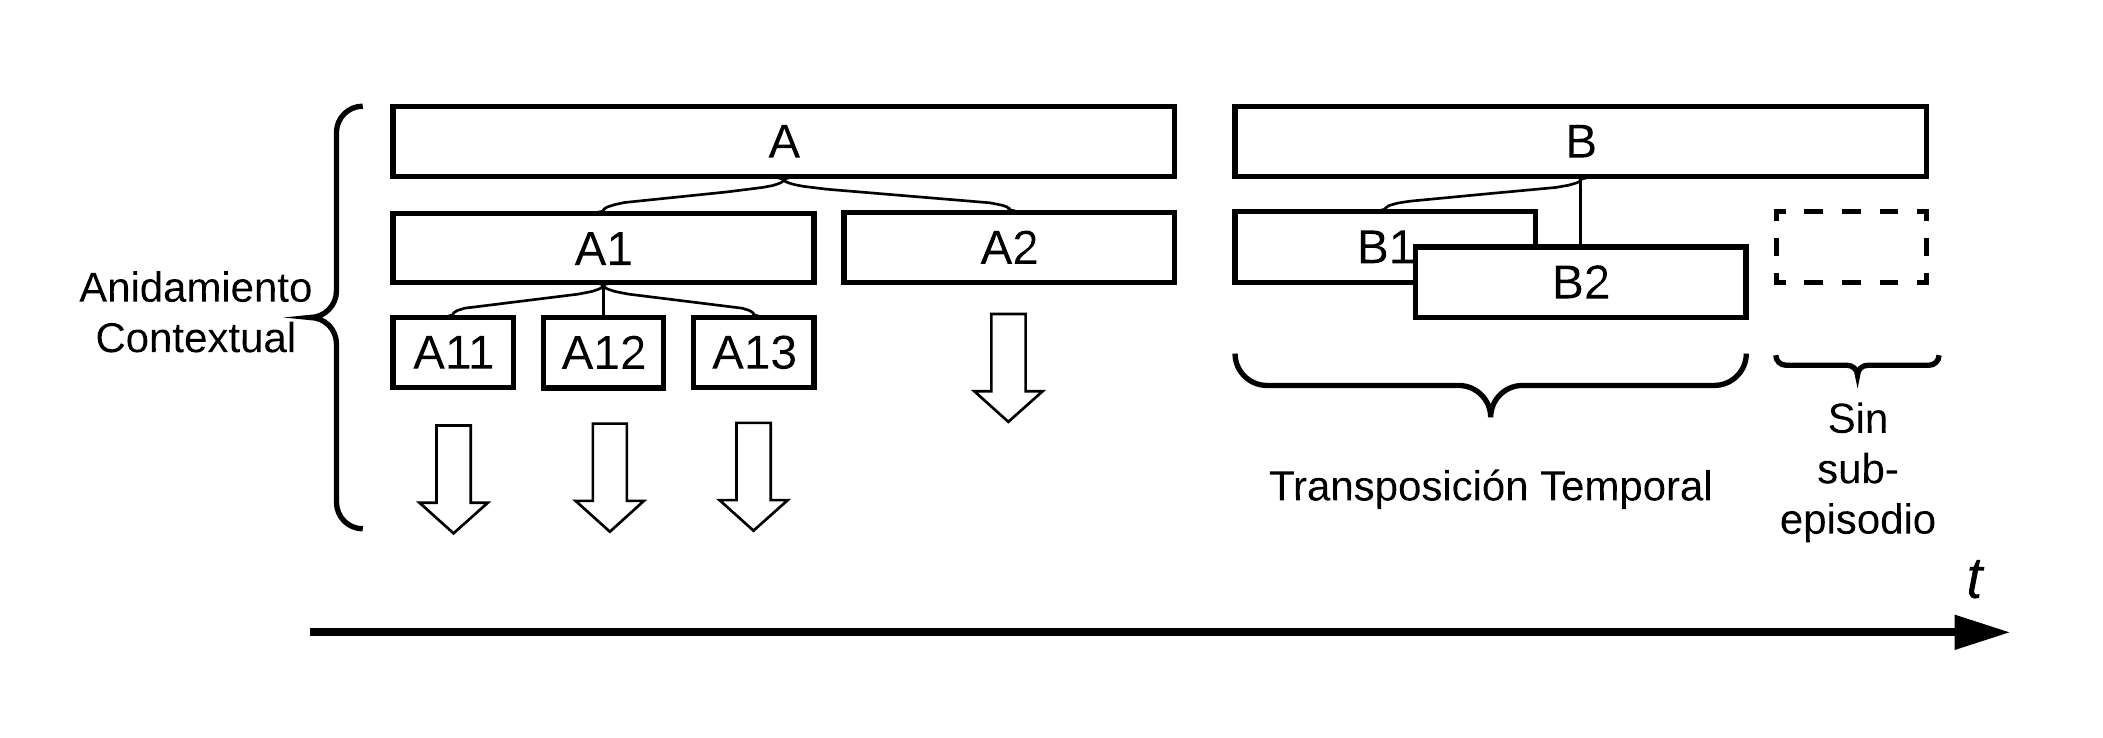
\includegraphics[width=\textwidth]{episodes.png}
	\caption[Concepto de anidamiento y transposición episódica.]
	{\small Diagrama temporal ejemplificando nociones de anidamiento y transposición episódica. Cada cuadro es un episodio identificado por el nombre indicado (\textit{A, B, A1}, \ldots). El tiempo transcurre horizontalmente hacia la derecha, por lo que \textit{A2} ocurre después de \textit{A1}, y \textit{B2} inicia después que \textit{B1}, pero ocurren simultáneamente por un periodo. Los episodios pueden ser anidados indefinidamente.}
	\label{img:episodes}
\end{figure}

% SOBRE TEMPORALIDAD
\ltmconcept{Temporalidad}
Para el árbol episódico es fundamental que cada episodio padre inicie antes que cualquiera de sus hijos, y termine después que todos ellos. Lo anterior es presentado en el diagrama de la Figura~\ref{img:episodes}, donde además se ejemplifica el caso de la transposición episódica, y que un padre puede tener lapsos de tiempo sin hijos asociados.

% SOBRE MANEJO DE INFORMACIÓN EN PADRES E HIJOS
\ltmconcept{Estrategia de almacenamiento}
Ya que un padre puede ser representado lógicamente por su conjunto de hijos, se decide utilizar una metodología de almacenamiento que no genere redundancia de información. Sólo las hojas del árbol son las encargadas de manejar la información semántica del episodio, lo que potencialmente corresponde a una gran cantidad de información. Asimismo, las hojas son encargadas de manejar la mayor cantidad de información episódica que sea posible. Las estrategias para esto serán explicadas en sus respectivas secciones. Por lo tanto, los nodos internos del árbol (en adelante, \textit{nodos}) manejan poca información y la mayor parte de sus datos puede ser calculada recursivamente a partir de sus hijos y de manera automática por el servidor.

% SOBRE EL CONTEXTO
\ltmconcept{Noción de contexto}
Es importante enfatizar que no basta que un episodio esté embebido temporalmente en otro para ser considerado un hijo. Pues a pesar de cumplir la condición de temporalidad, puede ocurrir el caso de que ambos episodios sean simultáneos (ver \RSlabel{12}), pero estén ligados a un contexto distinto. Por ejemplo, dado un episodio A (el robot está participando la competencia RoboCup - días de duración) y un episodio B (durante la competencia, el robot es utilizado para una tarea de uno de los estudiantes, lo que es considerado ajeno a la competencia); a pesar de que A contiene temporalmente a B, se puede decir que B pertenece a otro contexto y debe ser almacenado en un árbol distinto. Esta noción de contexto es importante, y es la razón por la que el servidor debe manejar una cantidad indefinida de árboles episódicos, cada uno identificado por su raíz. Debido lo anterior, cada episodio debe ser almacenado indicando quien es el padre asociado.



%% =============================================================================
%% =============================================================================
%% =============================================================================
\subsection{Contexto temporal: \textit{When}}\label{sec:design_ep_when}
%% =============================================================================
%% =============================================================================
%% =============================================================================

% SOBRE LOS REQUISITOS
\ltmconcept{Requisitos}
De acuerdo al requisito \RSlabel{03}, los episodios deben almacenar información que indique su contexto temporal (\textit{When}), es decir, cuándo  sucedió. Para esto, la única información de interés a almacenar son los instantes de tiempo que indican el fin y el inicio del episodio.

% SOBRE MANEJO DE INFORMACIÓN
\ltmconcept{Estrategia de almacenamiento}
En el caso de las hojas, basta utilizar los instantes de tiempo obtenidos al iniciar y finalizar el episodio. Sin embargo, para el caso de los nodos, se pueden seguir dos estrategias: Utilizar los instantes de tiempo iniciales y finales percibidos, o calcular automáticamente los tiempos de inicio y fin para ajustarse a los hijos. A pesar de que la segunda opción suena razonable, está asumiendo que siempre existirá un hijo para cada instante de tiempo de vida del padre, lo que puede no ser cierto. Por lo tanto, se deben manejar cuidadosamente los valores de tiempo de los padres, para asegurar que no son sobre-escritos por sus hijos, y para asegurar que los padres siempre contienen temporalmente a cada hijo.


%% =============================================================================
%% =============================================================================
%% =============================================================================
\subsection{Contexto espacial: \textit{Where}}\label{sec:design_ep_where}
%% =============================================================================
%% =============================================================================
%% =============================================================================

% SOBRE LOS REQUISITOS
\ltmconcept{Requisitos}
De acuerdo al requisito \RSlabel{04}, los episodios deben almacenar información que indique su contexto espacial (\textit{Where}), es decir, dónde sucedió. A continuación se explican las decisiones de diseño consideradas.

% SOBRE DURACIÓN DE EPISODIOS Y VECTORES
\ltmconcept{Desplazamiento durante episodios}
En primer lugar, dependiendo de la duración del episodio, el robot puede haber estado en más de un lugar durante ese periodo. Esto no es válido sólo para episodios nodo, sino que también para hojas, cuando éstas representan acciones de desplazamiento del robot. Luego, es importante que cada episodio registre cada uno de los lugares en los que ha estado el robot. El listado de lugares debe ser almacenado ordenadamente y con la hora asociada a cada desplazamiento, lo que es importante por dos motivos: permite calcular la secuencia de movimientos para los padres, y permite reconstruir la ruta del robot durante cada episodio. Para ello, la posición del robot puede ser consultada periódicamente en busca de cambios, para almacenar sólo los instantes que indiquen movimiento. 

% SOBRE USO DE AMBAS OPCIONES: Lugares y coordenadas
\ltmconcept{Estrategias de almacenamiento}
La información espacial puede ser manejada de dos maneras: se pueden almacenar los nombres de los lugares en donde el robot estuvo durante el episodio, o se puede almacenar la ubicación precisa del robot durante el episodio, mediante posiciones relativas a un sistema coordenado predefinido. La decisión sobre cual sistema utilizar depende mucho del contexto en el cual funciona el robot. Por ejemplo, en el caso de Bender, hay ocasiones en donde sólo es posible conocer su ubicación respecto a un sistema coordenado, mientras que en otras oportunidades, sólo se tiene conocimiento verbal de ésta. Luego, ya que no existe un consenso sobre que opción es la mejor, y para evitar limitar la usabilidad del sistema LTM, se decide dar soporte a ambas alternativas.


% OPCIÓN SEMÁNTICA
\ltmconcept{Estrategia 1 - Descripción}
Los nombres de lugares en los que estuvo el robot durante el episodio pueden ser almacenados utilizando vectores de \textit{strings}. Considerando el ambiente en donde puede desempeñarse un robot de servicio doméstico, se decide almacenar esta información en dos niveles de profundidad. El primer nivel corresponde a una descripción específica de la ubicación del robot (e.g., ``Comedor''), mientras que el segundo sirve para almacenar el nombre del área donde se encuentra la primera ubicación (e.g., ``Casa de John''), junto a otras de similar orden semántico. En el caso de los episodios nodo, se ha decidido calcular automáticamente toda esta información a partir de sus hijos.

% OPCIÓN COORDENADAS
\ltmconcept{Estrategia 2 - Coordenadas}
Similarmente al caso anterior, las coordenadas de lugares son almacenadas en vectores de puntos, junto con su hora y sistema de coordenadas asociados. Además, para cada punto se debe almacenar el nombre del mapa en donde se define el sistema coordenado. Ya que el proyecto está orientado a robots de servicio doméstico, se ha decidido implementar solamente ubicaciones en 2 dimensiones, es decir, cada punto sólo considera 2 valores numéricos. En el caso de los padres se sigue la siguiente estrategia: las posiciones son obtenidas a partir de sus hijos, se agrega un campo para almacenar la envoltura convexa de todas las posiciones, y se agrega un campo indicando el centroide de ésta. La envoltura convexa es agregada por motivos prácticos, pues puede ser utilizada para visualización y análisis del árbol episódico.



%% =============================================================================
%% =============================================================================
%% =============================================================================
\subsection{Memoria semántica: \textit{What}}\label{sec:design_ep_what}
%% =============================================================================
%% =============================================================================
%% =============================================================================

% REQUISITOS
\ltmconcept{Requisitos}
De acuerdo a los requisitos \RSlabel{01}, \RSlabel{02}, la memoria semántica (\textit{What}) ligada a un episodio permite describir `qué'' sucedió en él. Ésta debe poder  contener cualquier dato, por lo que no es posible establecer de antemano qué información y estructura debe ser utilizada, sino que ésto debe poder ser definido por el usuario. El requisito \RSlabel{07} (regla de flexibilidad episódica) establece que cada episodio debe permitir crear nuevos datos semánticos o actualizar los ya existentes. El requisito \RSlabel{10} (regla de perspectiva episódica) exige que al leer un episodio, éste pueda describir sus datos semánticos asociados, de acuerdo a la misma perspectiva que se tenía de ellos cuando el episodio fue ejecutado.

% SEPARACIÓN DE CONCEPTOS
\ltmconcept{Streams y entidades}
La memoria semántica maneja entidades conocidas por el robot e información sobre ellas. Por ejemplo, se puede definir la entidad ``persona'' y almacenar datos como su nombre, nacionalidad o la fecha de la última interacción registrada. Sin embargo, existe un tipo de información que no está asociada a alguna entidad en particular, correspondiente a datos en forma de flujos de información (\textit{streams}). Éstos permiten registrar secuencias de imágenes, sonido y otros conceptos basados en flujos de datos percibidos por el robot, especialmente los obtenidos directamente desde sus sensores. Otra característica de los \textit{streams}, es que a diferencia de las entidades, representan datos que no se desea actualizar posteriormente, pues almacenan una fotografía de lo percibido en el instante, la que generalmente es invariable. Entonces, se decide separar la memoria semántica en dos componentes, \textit{streams} y entidades, lo que permite diseñar estrategias de procesamiento adecuadas al funcionamiento de cada uno. 


% GENERALIZANDO MEMORIA SEMÁNTICA
\ltmconcept{Generalización}
Ya que los contenidos a almacenar deben poder ser definidos por el usuario, se establecen las siguientes decisiones de diseño. En primer lugar, el usuario debe definir que información utilizará, mediante uno o más mensajes de ROS. Segundo, a partir del requisito \RSlabel{18}, debe haber una conexión bidireccional entre los mensajes y los episodios, esto es válido tanto para \textit{streams} como entidades:
\begin{itemize}
\item Mensajes deben tener una referencia al identificador del episodio relacionado.
\item Mensajes deben definir un campo para almacenar su identificador único, el que debe ser utilizado por el episodio.
\end{itemize}

% SOBRE PLUGINS
\ltmconcept{Sistema de plugins}
Se decidió utilizar un sistema basado en plugins para manejar los mensajes ROS definidos por el usuario. De esta manera, se delega al usuario la implementación de los algoritmos para adquisición de la  información semántica y procesamiento de ésta. El diseño del servidor LTM en la Sección~\ref{sec:design-server} especifica que funcionalidades deben ser implementadas por plugins destinados a \textit{streams} o entidades. 

% SOBRE STREAMS
\ltmconcept{Datos semánticos - Streams}
Los \textit{streams} corresponden a flujos de datos generalmente invariables, relacionados a un episodio según sus tiempos de inicio y fin. Existen 3 metodologías para almacenar los \textit{streams}, con ventajas y desventajas. En cada caso, no se requiere almacenar datos cuando no hay episodios activos:
\begin{enumerate}
	\item Cada \textit{stream} contiene sólo 1 dato semántico, por lo que no tiene duración y es asociado a un instante de tiempo. Esta estrategia es ideal funcionalmente, pero ya que la tasa de mensajes a almacenar puede ser alta, en la práctica esta solución es costosa en términos de consultas a la base de datos.
	\item Mantener 1 \textit{stream} por cada episodio, con tiempos de inicio y fin idénticos a los del episodio relacionado. Tiene la desventaja de almacenar información duplicada cuando existe traslape temporal de episodios.
	\item Similar a la estrategia anterior, pero subdividiendo el \textit{stream} cuando hay traslape de episodios. Evita la duplicación de información, pero complica la mantención de la base de datos.
\end{enumerate}

Para acotar el trabajo, y bajo la suposición de que en la práctica existen pocos episodios traslapados, se escoge la segunda estrategia. Entonces, cada episodio puede estar asociado a un \textit{stream} de cada tipo, y a su vez, cada \textit{stream} puede contener uno o más datos. El servidor debe proveer notificaciones para indicar el inicio y fin de un episodio, mientras que el usuario debe definir su estrategia para adquirir datos durante ese lapso de tiempo. Por ejemplo, en el caso de un \textit{stream} de imágenes representando la visión del robot, y cuyo fin sólo sea de visualización a futuro, el usuario podría almacenar una imagen cada 3 segundos. 

Según la cantidad de plugins a utilizar y la periodicidad de recopilación de información, el espacio de disco requerido para almacenar los mensajes puede ser agotado rápidamente. Para solucionar esto hay 3 alternativas. En primer lugar, se puede expandir la memoria disponible, lo que no es una solución real. En segundo lugar, está el ``olvido'' de información, mediante la eliminación de datos antiguos (posiblemente previo respaldo en otra máquina) o eliminar datos intercaladamente. La tercera opción es la degradación de información, para lo que cada usuario debe implementar un algoritmo que disminuya el tamaño de sus mensajes (e.g., disminuyendo la resolución o cantidad de las imágenes del episodio). Ya que las dos primeras opciones pueden ser ejecutadas manualmente por el usuario, se ha decidido utilizar la degradación de mensajes. Esta estrategia puede ser aplicada automáticamente a mensajes antiguos y de baja relevancia episódica.

% SOBRE ENTIDADES
\ltmconcept{Datos semánticos - Entidades}
El usuario debe definir cada tipo de entidad disponible a través un mensaje ROS. Cada tipo (e.g., ``persona'') puede tener muchas instancias (e.g., ``Carl'' y ``Lenny''). A diferencia de los \textit{streams}, las entidades manejan datos modificables, lo que introduce dos condiciones:
\begin{itemize}
\item Su modelo de datos debe soportar el requisito \RSlabel{07} al crear nuevas instancias o modificar una ya existente.
\item El modelo de datos debe soportar el requisito \RSlabel{10}, por lo que cada episodio debe almacenar referencias a las instancias modificadas y los cambios aplicados.
\end{itemize}

Las instancias de una entidad y sus modificaciones no están ligadas a un episodio particular, sino que a los episodios activos durante el registro la modificación. Entonces, es posible registrar cambios a entidades a pesar de no haber episodios activos.


%% =============================================================================
%% =============================================================================
%% =============================================================================
\subsection{Relevancia generalizada}
%% =============================================================================
%% =============================================================================
%% =============================================================================

% RELEVANCIA GENERALIZADA
\ltmconcept{Requisitos}
De acuerdo a los requisitos \RSlabel{19}-\RSlabel{20}-\RSlabel{21}, los episodios deben almacenar información de relevancia episódica. Estos indicadores son importantes al momento de buscar episodios, para poder ordenarlos de acuerdo a una medida de importancia, y así tener una pista sobre cuales enfocar la atención. El sistema debe soportar, al menos, la noción de relevancia histórica y emocional, considerando que en un futuro se podrían agregar otros indicadores de relevancia. También, el sistema debe proveer un indicador generalizado, capaz de representar la relevancia global del episodio, mediante un solo indicador numérico que unifique las sub-relevancias.

% MANEJO DE INDICADORES
\ltmconcept{Estrategia de almacenamiento}
Entonces, se define la siguiente estrategia de almacenamiento. Cada tipo de indicador debe proveer un valor numérico en el rango $[0, 1]$, que represente la importancia del episodio de acuerdo a su perspectiva. Un valor de 0 significa que el episodio no es relevante, mientras que el valor 1 es utilizado para indicar que el episodio es muy importante. Utilizando el formato anterior, se construye el indicador de relevancia generalizada a partir de todas las sub-relevancias definidas para el episodio. Este indicador debe ser actualizado cada vez que una sub-relevancia sea modificada o ingresada.

% COMPUTO BASADO EN ALGORITMO X
\ltmconcept{Cómputo}
Este proyecto sólo considera dos sub-indicadores, histórico y emocional, por lo que se decidió utilizar la metodología propuesta por Dood et al y explicada en la Sección~\ref{sec:theory-modulation}.


%% =============================================================================
%% =============================================================================
%% =============================================================================
\subsection{Relevancia emocional}\label{sec:design_ep_rel_emo}
%% =============================================================================
%% =============================================================================
%% =============================================================================

% RELEVANCIA EMOCIONAL
\ltmconcept{Requisitos}
El requisito de sistema \RSlabel{19} exige el manejo del concepto de relevancia emocional, como un medio para almacenar las emociones ``que siente'' el robot durante un episodio, en conjunto a un indicador de la intensidad de éstas.


% ABSTRACCIÓN DEL SISTEMA DE EMOCIONES
\ltmconcept{Abstracción del sistema emocional}
Según se revisó en la Sección~\ref{sec:theory-modulation}, existen diversos sistemas para la generación de emociones y no existe una metodología única para su implementación: Cada sistema es alimentado con datos diferentes, utilizan algoritmos distintos y proveen salidas distintas. Debido a la generalidad esperada para el proyecto, se propone la siguiente estrategia para la abstracción del sistema emocional a utilizar, que permite delegar la implementación al usuario:
\begin{itemize}
\item Se define un conjunto de 8 emociones base, a partir de las emociones primarias propuestas por Plutchik (Ver Sección~\ref{sec:theory-modulation}).
\item Se debe almacenar el nivel de intensidad percibido durante un episodio, para cada una de las 8 emociones.
\item Se utilizará un sistema de plugins, donde el usuario debe implementar el mapeo entre las salidas de su sistema emocional, a la combinación de emociones base disponibles para un episodio.
\end{itemize}

% CAMPOS REQUERIDOS
\ltmconcept{Estrategia de almacenamiento}
Las 8 emociones definidas deben seguir el estándar definido para la representación de relevancias, con valores en el rango $[0, 1]$ indicando la intensidad asociada. La relevancia emocional de cada episodio se asocia a la emoción cuya intensidad sea la de mayor valor. Para el caso de episodios nodo, el registro emocional es calculado automáticamente a partir de los hijos, almacenando los valores máximos para cada emoción.

% METADATOS
\ltmconcept{Metadatos}
Además, para simplificar la introspección de episodios a futuro, se decide agregar metadatos que indican el software emocional utilizado y su versión. Es importante enfatizar que cada metadato sólo debe ser utilizado para introspección y no tienen influencia en el cálculo de las relevancias.


%% =============================================================================
%% =============================================================================
%% =============================================================================
\subsection{Relevancia histórica}\label{sec:design_ep_rel_hist}
%% =============================================================================
%% =============================================================================
%% =============================================================================

% SOBRE RELEVANCIA HISTORICA
\ltmconcept{Requisitos}
El requisito \RSlabel{20} exige el manejo del concepto de relevancia histórica, como un medio para indicar la importancia de un episodio, según su edad en la base de datos. 

% ALMACENAMIENTO
\ltmconcept{Estrategia de almacenamiento}
Siguiendo el estándar definido para representación de relevancias, se utiliza un valor numérico en el rango $[0, 1]$, que indica el estado de envejecimiento del episodio. Este valor siempre debe ser inicializado en 1, para decaer hacia 0 con el paso del tiempo.

% MANEJO AUTOMÁTICO DE DATOS HISTÓRICOS
\ltmconcept{Actualización automática}
El valor de la relevancia debe ser manejado automáticamente por el sistema LTM. Se propone disminuir el indicador, según el algoritmo de decaimiento presentado por Dood et al. (ver Sección~\ref{sec:theory-modulation}). Ya que se espera almacenar una gran cantidad de episodios, se propone discretizar la función de decaimiento. Los episodios deben ser actualizados en lapsos cada vez más espaciados en el tiempo (e.g., primero cada 1 día, luego 1 vez a la semana, cada 1 mes, cada 1 año), lo que permite acotar el esfuerzo computacional dedicado a las actualizaciones.


%% =============================================================================
%% =============================================================================
%% =============================================================================
\subsection{Datos para introspección}
%% =============================================================================
%% =============================================================================
%% =============================================================================

% SOBRE RAZONAMIENTO
\ltmconcept{Metadatos}
El último conjunto de datos considerado para un episodio es denominado \textit{Metadatos}. Éstos no están ligados a algún requerimiento de software, por lo que no son formalmente necesarios, sin embargo, permiten almacenar datos útiles para la implementación LTM, y sirven para conocer información sobre el software utilizado durante el almacenamiento de cada episodio. Los \textit{Metadatos} tienen como finalidad ser de utilidad al resolver problemas relacionados al sistema LTM, y para cuando los usuarios deseen conocer el contexto de software sobre el cual fue generado el episodio.


%% =============================================================================
%% =============================================================================
%% =============================================================================
\subsection{Limitantes y trabajo futuro}
%% =============================================================================
%% =============================================================================
%% =============================================================================

% SOBRE LIMITANTES DEL DISEÑO Y TRABAJO FUTURO
A continuación se presenta un conjunto de limitantes conocidas del diseño episódico desarrollado, las que pueden ser consideradas como parte del trabajo futuro del proyecto.

% SOBRE COMPLETITUD Y LAPSOS EN BLANCO..
\ltmconcept{Ausencia de hijos}
Este problema fue explicado parcialmente en la Sección~\ref{sec:design_ep_when}, y aparece con padres cuyo rango temporal no es cubierto completamente por sus hijos. Esto puede suceder cuando el usuario decide no almacenar algunos episodios hoja, pues los considera poco relevantes. El efecto de ésto, es que los padres podrían contar con información incompleta al calcular datos a partir de sus hijos. Se puede argumentar que, ya que el usuario considera que los subepisodios eran irrelevantes, entonces la información perdida también lo es. Sin embargo, por motivos de introspección, puede ser de interés almacenar los datos de \textit{streams} asociados a los periodos temporales perdidos.

\ltmconcept{Episodios de larga duración}
A pesar de que el diseño permite episodios de duración indefinida, en la práctica es raro que el robot funcione por periodos prolongados. Luego, los episodios cuyo fin es dar un contexto temporal a un árbol episódico no pueden ser almacenados directamente (e.g., cuando el robot está participando en una competencia de 4 días de duración). A pesar de lo anterior, el diseño permite la introducción manual de episodios de larga duración, sin tener que mantener en funcionamiento el robot durante todo el periodo.

\ltmconcept{Memoria emocional detallada}
Ya que el diseño apunta a ser lo suficientemente genérico, la información emocional que se puede exigir es acotada. El formato permite almacenar los datos justos para la asignación de relevancias, pero a la vez, limita las consultas posibles sobre las emociones del robot en un episodio. Particularmente, en episodios de larga duración sería interesante conocer la secuencia (ordenada) de emociones, o las causas de éstas. A pesar de que el diseño no almacena información al respecto, si permite definir una forma alternativa de almacenar tales datos. Se puede crear una entidad ``Robot'' con campos asociados a sus emociones, para así, llevar un registro detallado de lo que se necesite.

\ltmconcept{Ubicación del robot duplicada o no útil}
Se cree que el formato propuesto para el campo \textit{Where} se ajusta a los requerimientos de un robot doméstico, sin embargo, se identifican dos problemas. Por un lado, la naturaleza de la ubicación del robot no depende de un episodio, sino que es información desacoplada de éste, similar al funcionamiento de una entidad. Esto genera duplicación de la información en caso de traslape episódico. Por otro lado, se cree que el formato es lo suficientemente genérico, pero pueden haber casos donde la información de localización sea conveniente almacenarla en otros términos. En un trabajo futuro se podría modificar el diseño, para manejar el campo \textit{Where}  de manera similar al caso de las entidades, donde cada usuario defina los datos que desea almacenar, y evitando redundancia de información.

%% =============================================================================
%% =============================================================================

%% =============================================================================
%% =============================================================================

%% =============================================================================
%% =============================================================================

%% =============================================================================
%% =============================================================================
%% =============================================================================
\section{Diseño del Modelo de Datos}\label{sec:data_model_design}
%% =============================================================================
%% =============================================================================
%% =============================================================================

Es esta sección se presentan las decisiones sobre el diseño del modelo de datos a utilizar para el proyecto. En primer lugar, se revisan las consideraciones sobre la base de datos escogida: \textit{MongoDB}. Luego, se describe el manejo de mensajes episódicos y sus datos semánticos asociados: \textit{streams} y entidades.


%% =============================================================================
%% =============================================================================
%% =============================================================================
\subsection{Base de datos}
%% =============================================================================
%% =============================================================================
%% =============================================================================

% SOBRE SELECCIÓN DE MONGO DB
\ltmconcept{MongoDB}
De acuerdo al diseño de los mensajes episódicos, la implementación del sistema LTM requiere el manejo de datos aleatorios, representados mediante mensajes de ROS que debe definir el usuario. Además, el sistema debe permitir modificar la representación de tales mensajes a futuro y soportar el almacenamiento de datos binarios. Se decidió utilizar la base de datos no relacional \textit{MongoDB}, presentada en la Sección~\ref{sec:mongodb}. 

La decisión sobre el uso \textit{MongoDB} se basa en tres razonamientos principales. Primero, \textit{MongoDB} ya es de uso extendido en la comunidad, por lo que ya ha sido probada y está disponible en muchos robots de servicio domésticos, evitando agregar dependencias extra a tales proyectos. Además, la interfaz ROS para ésta es considerada estable, al menos hasta el año 2023.  Finalmente, \textit{MongoDB} se ocupa actualmente en el robot Bender. Así, se minimizan los problemas de dependencias y compatibilidad a futuro.


% SOBRE SEPARACIÓN DE COLECCIONES
\ltmconcept{Colecciones}
Debido al funcionamiento de \texttt{warehouse\_ros\_mongo}, cada mensaje ROS debe ser asociado a una colección distinta. Particularmente, una colección será destinada al almacenamiento de episodios, mientras que cada mensaje definido por el usuario será asociado a una colección diferente. En primera instancia, la base de datos no relacional permitiría almacenar todos los mensajes en la misma colección, pero la separación de cada tipo de dato en colecciones diferentes es conveniente por las siguientes razones:
\begin{itemize}
\item Permite optimizar las consultas simples a la base de datos, que no requieran acceder a toda la memoria semántica asociada.
\item Se evita propagar problemas al registro de episodios, cuando se presenten fallos en los plugins de memoria semántica implementados por el usuario.
\item Ya que el sistema debe soportar una cantidad indefinida de mensajes ROS elegidos por el usuario, se evita saturar el registro de episodios con mensajes que, una vez agrupados, superen el límite de tamaño (16MB) permitido a cada elemento de una colección.
\end{itemize}

% REQUISITO DE MODIFICACIÓN DE REPRESENTACIÓN
\ltmconcept{Modificación de mensajes semánticos}
El requisito \RSlabel{14} especifica que el servidor debe permitir modificar la representación de los mensajes episódicos almacenados. Esto puede suceder porque el usuario decide agregar/quitar campos al mensaje, o porque una dependencia del mensaje fue actualizada. La implementación debe soportar la migración desde la estructura antigua a la nueva.

%% =============================================================================
%% =============================================================================
%% =============================================================================
\subsection{Colección de episodios}
%% =============================================================================
%% =============================================================================
%% =============================================================================

Todos los episodios, definidos por su mensaje ROS, serán almacenados en la colección \texttt{episodes}. De acuerdo a los requisitos \RSlabel{05} y \RSlabel{22}, cada episodio debe ser indexado al menos por los campos \textit{What}, \textit{When}, \textit{Where}, las relevancias emocionales y sus campos internos. En el caso de \textit{What}, las entidades y \textit{streams} también deben ser indexados, y queda a criterio del usuario cuales campos son de interés para cada concepto.

%% =============================================================================
%% =============================================================================
%% =============================================================================
\subsection{Colecciones de streams}
%% =============================================================================
%% =============================================================================
%% =============================================================================

\ltmconcept{Colección}
Según se explicó anteriormente, cada \textit{stream} definido por el usuario es asociado a una colección de \textit{MongoDB} propia. El nombre de cada colección lleva el prefijo \texttt{stream:}, seguido de un identificador definido por el usuario.

\ltmconcept{Estrategia}
Por cada episodio a almacenar se genera un \textit{stream} de cada tipo disponible, para ser almacenado en su colección respectiva. Esto se ejemplifica en la Figura~\ref{img:episodes-and-semantic-data}, mediante un diagrama comparando la relación entre un episodio y los datos semánticos percibidos, de acuerdo al diseño episódico descrito en la Sección~\ref{sec:design_ep_what}.

\begin{figure}[!h]
	\centering
	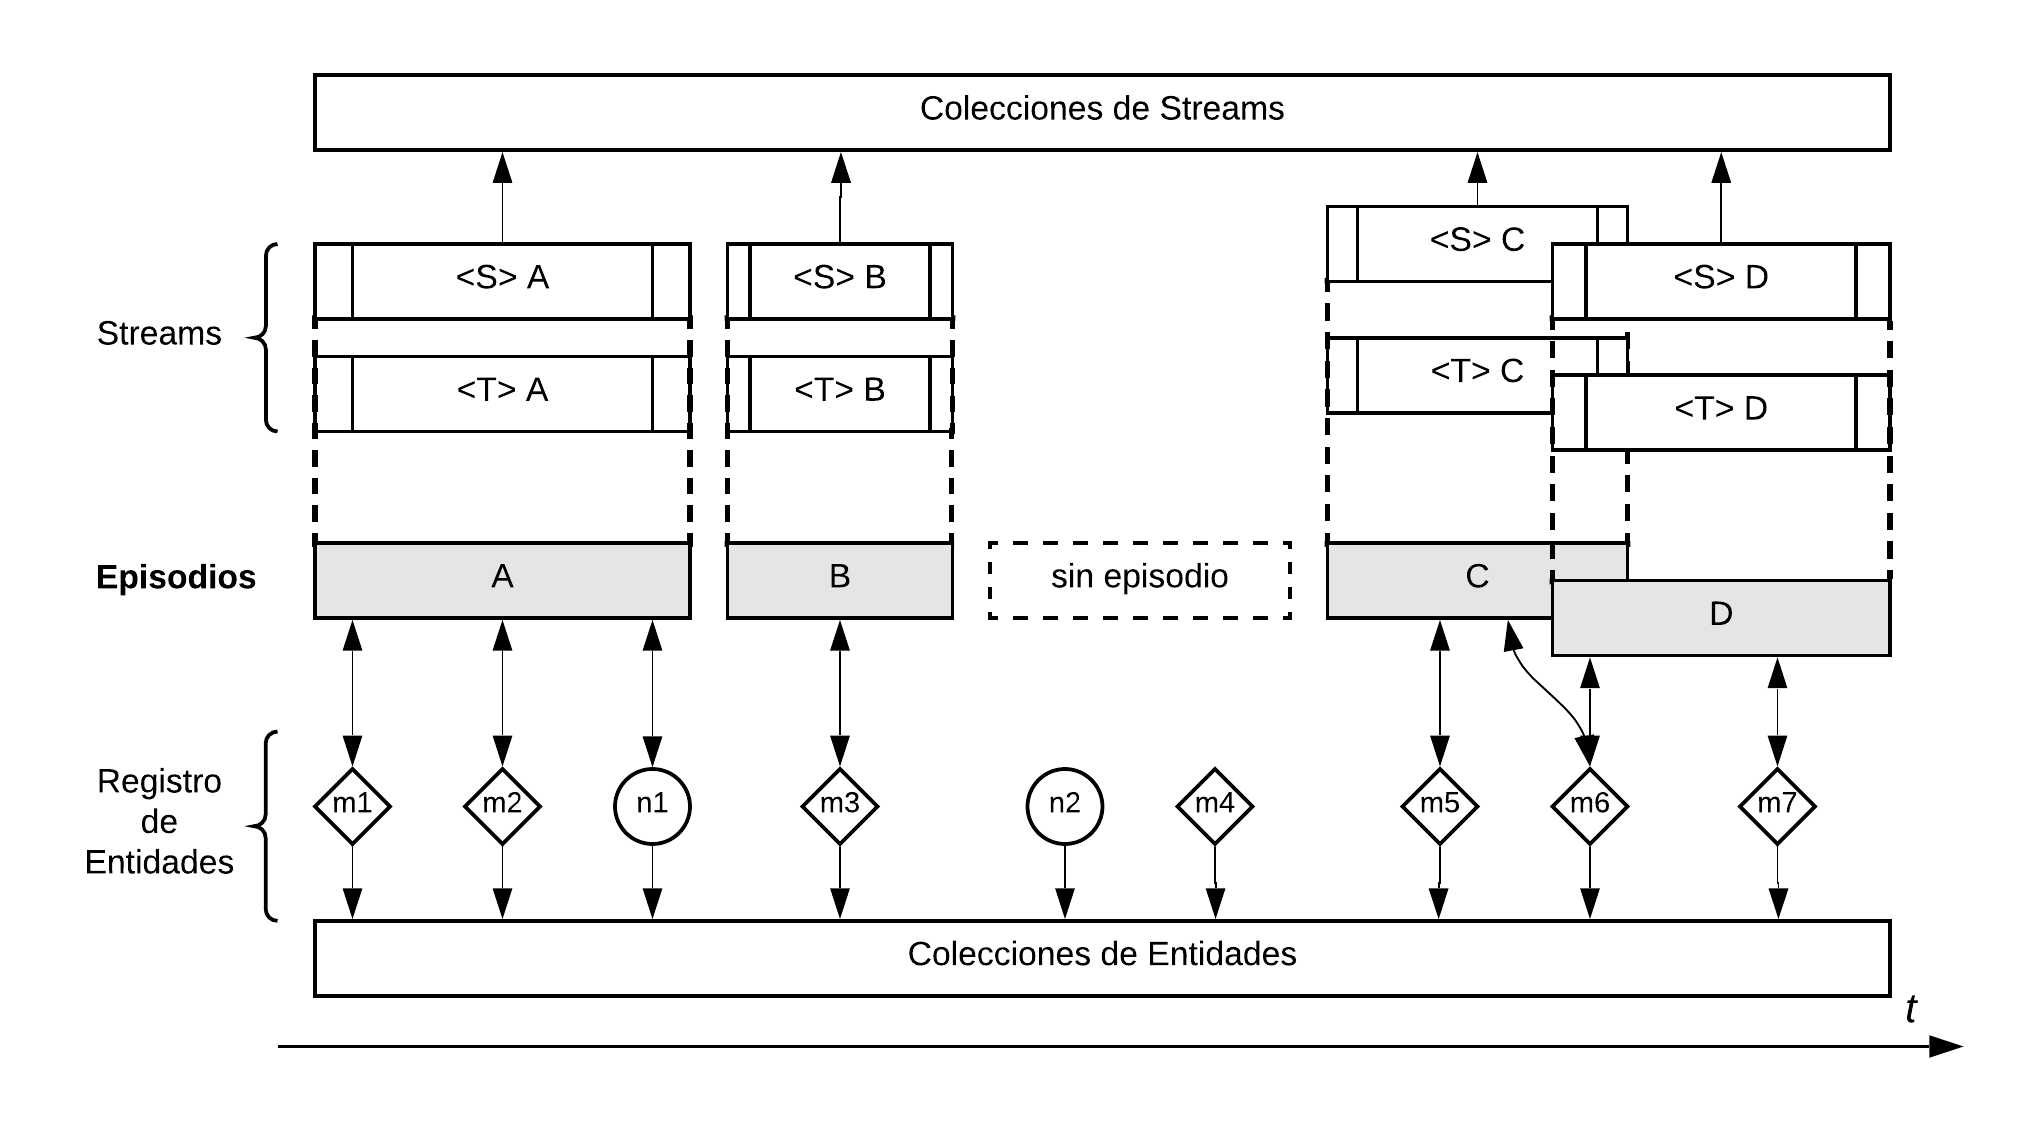
\includegraphics[width=\textwidth]{episodes-and-semantic-data.png}
	\caption[Funcionamiento de \textit{streams} y entidades respecto a los episodios.]
	{\small Funcionamiento de \textit{streams} y entidades respecto a los episodios. \texttt{\textless S\textgreater} y \texttt{\textless T\textgreater} hacen referencia a 2 tipos de \textit{streams}, mientras que \texttt{$m_1\ldots m_7$} (rombos) y \texttt{$n_1, n_2$} (círculos) son notificaciones sobre cambios a las entidades \textit{m} y \textit{n}. Un \textit{stream} de cada tipo es asociado a cada episodio, incluso en caso de transposición. Cada notificación sobre entidades es asociada a todo episodio activo. En caso de no haber episodio, no se almacenan \textit{streams}, pero si se registran los cambios en entidades.}
	\label{img:episodes-and-semantic-data}
	\end{figure}


\ltmconcept{Indexado}
Por lo general, los campos de un \textit{stream} no requieren ser indexados, ya que es conveniente almacenarlos de manera binaria. Sin embargo, durante la implementación del plugin asociado, el usuario puede decidir añadir metadatos para indexar campos convenientes. La utilidad de ésto, es que permitirá agregar nuevos términos de comparación para las consultas a la base de datos. Luego, se tienen dos formas de acceder a un \textit{stream} en particular; mediante su mensaje episódico asociado, o a través de los metadatos definidos por el usuario.

\ltmconcept{Tamaño del mensaje}
El límite de tamaño para cada mensaje ROS a almacenar es de $16 MB$, lo que impone una cota superior a la cantidad de datos que pueden ser almacenados por cada episodio. Según se describe en la Sección~\ref{sec:mongodb}, \textit{MongoDB} provee estrategias de almacenamiento para evitar este límite.

%\todoimprove{Por ejemplo, esto permitiría almacenar hasta $N$ imágenes a color de cierto tamaño, o $M$ de ellas en escala de grises.}


%% =============================================================================
%% =============================================================================
%% =============================================================================
\subsection{Colecciones de entidades}
%% =============================================================================
%% =============================================================================
%% =============================================================================

\ltmconcept{Colección}
Cada mensaje ROS definido por el usuario para representar una entidad de la memoria semántica, es asociado a una colección de \textit{MongoDB} propia. El nombre de cada colección lleva el prefijo \texttt{entity:}, seguido de un identificador definido por el usuario. 

\ltmconcept{Flexibilidad}
El modelo debe considerar un identificador único para indicar la instancia de cada entidad. Así, cuando un episodio registra actualizaciones de una instancia particular, modifica su entrada en la colección correspondiente.

\ltmconcept{Perspectiva}
Para soportar este concepto se requiere poder reconstruir el estado de una instancia en cada instante de tiempo desde su creación. Este es un requisito común para una base de datos, denominado \textit{Audit Trail}. La solución propuesta para el problema es la siguiente:
\begin{itemize}
\item Por cada entidad (mensaje ROS) se deben mantener 2 colecciones en la base de datos.
\item Las primera colección almacena un historial de las modificaciones a cada instancia de la entidad. Cada entrada debe indicar el tiempo de ocurrencia, tener referencias a los episodios asociados e indicar los cambios modificados.
\item La otra colección almacena el estado actual de cada instancia de la entidad, lo que es equivalente a aplicar su historial de cambios desde el comienzo. Esta colección tiene el propósito de agilizar consultas que sólo requieran los conocimientos actuales de cada instancia.
\end{itemize}
Ya que \texttt{warehouse\_ros\_mongo} sólo permite almacenar un tipo de mensaje ROS por colección, la destinada a almacenar los cambios es subdividida en dos colecciones:
\begin{itemize}
\item La primera almacena un mensaje ROS del mismo tipo que la entidad, y sirve para indicar los cambios registrados. Su nombre utiliza el prefijo \texttt{entity:} y el sufijo \texttt{.trail}.
\item La segunda almacena un mensaje ROS con los metadatos necesarios para mantener el historial. Su nombre utiliza el prefijo \texttt{entity:} y el sufijo \texttt{.meta}.
\end{itemize}

\ltmconcept{Estrategia}
Con la finalidad de mantener la consistencia del historial de entidades, se deben almacenar todos los cambios recolectados para una entidad, a pesar de que no haya un episodio activo. Sin embargo, cada registro debe tener referencias a los episodios activos durante el instante de su recolección, y a su vez, cada episodio debe tener referencias a tales registros. Lo anterior es ejemplificado en el diagrama de la Figura~\ref{img:episodes-and-semantic-data}.

\ltmconcept{Indexado}
Se delega al usuario la definición de los campos de interés para el indexado de su mensaje. Estos campos estarán disponibles para realizar consultas episódicas al servidor. Sin embargo, para enriquecer las búsquedas de episodios, los metadatos del registro histórico deben tener vectores con los nombres de los campos modificados, campos creados, y campos eliminados. Los 3 vectores deben estar indexados.


%% =============================================================================
%% =============================================================================
%% =============================================================================
\subsection{Consultas al modelo}
%% =============================================================================
%% =============================================================================
%% =============================================================================

De acuerdo a los requisitos \RSlabel{06} y \RSlabel{17}, el modelo debe soportar operaciones CRUD sobre los episodios y mensajes semánticos almacenados. Las operaciones deben permitir filtrar los episodios mediante condiciones de \{igualdad, mayor/menor que, pertenencia a arreglos\} sobre los campos indexados. Se debe dar soporte para comparaciones entre los siguientes tipos de dato primitivos de ROS: \{\texttt{bool}, \texttt{int}, \texttt{float}, \texttt{string}\} y condiciones de pertenencia a arreglos de esos tipos.

A continuación se describe la estrategia de procesamiento para las consultas CRUD que debe soportar el sistema. En cada caso se enfatizan las reglas a seguir para mantener la consistencia del modelo de datos.

\subsubsection{Operaciones de inserción (Create)}
%% =============================================================================

\ltmconcept{Episodios}
La inserción de episodios se hace en un proceso de dos etapas:
\begin{enumerate}
\item  Al inicio del episodio se declara la creación de este al servidor, el que proveerá un identificador disponible para su registro. Si el usuario indica que se trata de un episodio hoja, el servidor notifica a los plugins relacionados para que recopilen la información episódica y semántica requerida.
\item  Al finalizar el episodio, el usuario debe indicar la referencia al padre. Éste proceso notifica a los plugins para que finalicen la recopilación de información y se almacene el mensaje episódico y el \textit{stream} asociado.
\end{enumerate}
Tras la inserción del episodio se deben actualizar todos los padres, hasta llegar a la raíz.

Los requisitos no lo exigen, pero en caso de dar soporte para la inserción de episodios pasados, no se deben ejecutar los plugins episódicos ni semánticos. La información sobre relevancia emocional y posición debe ser entregada por el usuario. El \textit{stream} debe ser insertado manualmente por el usuario. Se deben registrar automáticamente las entidades que calcen con el lapso de tiempo designado. Análogamente, se debe actualizar el árbol episódico, hasta llegar a la raíz.

\ltmconcept{Streams}
Para la inserción de \textit{streams} se debe indicar el episodio asociado e incluir la referencia del \textit{stream} al episodio. En caso de ya existir un \textit{stream} del mismo tipo asociado al episodio, se sobreescribe la referencia y se elimina el antiguo de su colección. Además, es necesario que los tiempos de inicio y fin del mensaje estén dentro de los límites temporales definidos por el episodio.

\ltmconcept{Entidades}
Los requisitos \RSlabel{07} (flexibilidad) y \RSlabel{10} (perspectiva) establecen dos operaciones de inserción sobre entidades: creación de una nueva instancia y la modificación de una instancia ya existente, mediante la inserción de un nuevo registro en el historial. Ambas operaciones son requeridas para registros obtenidos en el instante actual. Ya que la creación de una nueva instancia se puede ver como un caso particular de modificación, sólo se detallará la estrategia del último caso:
\begin{itemize}
\item El nuevo registro debe indicar la fecha de creación, un identificador único del historial y una referencia a la instancia que modifica/crea.
\item Se debe modificar/crear la instancia en la colección que mantiene los datos actualizados.
\item La inserción del registro sólo debe almacenar los datos que fueron modificados, agregados o eliminados. La información que se mantuvo estática no debe ser registrada.
\item Se deben agregar referencias bidireccionales a los episodios cuyo lapso de vida contenga al registro.
\end{itemize}

No es necesario dar soporte para crear nuevos registros del historial de entidades, asociados a un tiempo pasado. En caso de hacerlo, se debe seguir una estrategia similar a la anterior, pero además modificando recursivamente los registros adyacentes (temporalmente), para mantener la consistencia del historial.

\ltmconcept{API ROS} Las operaciones de inserción de \textit{streams} y entidades son manejadas automáticamente por el sistema LTM, por lo que no es necesario proveer una API para ello. Por otro lado, si se requiere una API para las operaciones de registro e inserción de episodios.

\subsubsection{Operaciones de lectura (Read)}
%% =============================================================================

\ltmconcept{Etapas de consulta}
Para evitar sobrecargar el ancho de banda de red, con respuestas a consultas que retornen muchos episodios o datos semánticos, se diseñan las operaciones de lectura en 2 etapas. Primero, se obtienen los identificadores de los mensajes de interés mediante una condición que provee el usuario. Luego, se puede acceder a los episodios, \textit{streams} y entidades mediante servicios ROS, encargados de retornar mensajes para los identificadores escogidos.

\ltmconcept{Filtro de mensajes}
La búsqueda de mensajes según condiciones es considerada por el requisito \RSlabel{06}.
Para evitar limitar las consultas que puede realizar el usuario sobre la base de datos y para simplificar el diseño, se decide utilizar el sistema de condiciones nativo de MongoDB. Así, es posible aplicar filtros complejos a las consultas, basados en todos los campos disponibles de cada documento. Sin embargo, las consultas sólo pueden ser aplicadas a una colección a la vez. Algunas de las condiciones que provee MongoDB son: igualdad, mayor qué (y derivados), pertenencia a un arreglo y agrupamiento lógico mediante condiciones \textit{AND} y \textit{OR}.

\ltmconcept{Episodios}
Se debe proveer un servicio para filtrar episodios de acuerdo a una condición basada en los metadatos disponibles. El servicio debe retornar los identificadores de los episodios que calcen con la condición, junto a los identificadores de los \textit{streams} y entidades asociadas. Además, se debe proveer un servicio para obtener episodios de acuerdo a su identificador.

\ltmconcept{Streams}
De manera similar, se debe proveer un servicio para filtrar \textit{streams} de acuerdo a una condición basada en sus metadatos. El servicio debe retornar los identificadores de los mensajes que cumplan la condición y sus episodios asociados. Además, se debe proveer un servicio para obtener \textit{streams} mediante su identificador.

\ltmconcept{Entidades}
En el caso de las entidades, el filtro debe poder ser aplicado a la colección de entidades actuales y al historial de cambios. La consulta al historial debe permitir filtrar mediante los nombres de los campos modificados, añadidos u olvidados en cada registro. En ambos casos, se deben retornar los identificadores de las entidades o registros que calcen con la condición, sumado a los de los episodios asociados.

Además, se debe proveer un servicio para obtener una entidad según su identificador. Sin embargo, para cumplir con el requisito \RSlabel{10} (perspectiva), la consulta debe permitir indicar una fecha, para retornar la entidad de acuerdo al conocimiento obtenido hasta el momento.

\ltmconcept{API ROS}
De acuerdo a lo anterior, se debe proveer una API ROS para realizar consultas con condiciones en el formato de MongoDB, para las colecciones de episodios, \textit{streams} y entidades. Además, se deben proveer servicios ROS para obtener episodios, entidades y \textit{streams} según sus identificadores.

\subsubsection{Operaciones de actualización (Update)}
%% =============================================================================

\ltmconcept{Episodios}
De acuerdo al requisito \RSlabel{08} (más detalle en \RStachowicz{4}), los episodios son únicos y sólo tienen una instancia para ser aprendidos. Entonces, a pesar de ser útil, no es necesario proveer servicios para la actualización de episodios. En el caso de hacerlo, se deben modificar todos los nodos padres, hasta llegar a la raíz. En caso de modificar el intervalo de tiempo, se deben actualizar las referencias bidireccionales con las entidades ya existentes. Al acortar el intervalo de tiempo, se debe modificar el \textit{stream} asociado, para eliminar mensajes sobrantes.

\ltmconcept{Streams} De la misma manera, ya que los \textit{streams} hacen referencia a datos estáticos, no es necesario proveer esta funcionalidad para ellos. Sólo tiene sentido actualizar el intervalo de tiempo del mensaje cuando el de su episodio relacionado sea modificado.

\ltmconcept{Entidades}
Por otro lado, el requisito de flexibilidad \RSlabel{07} exige que las entidades deban soportar operaciones de actualización. Éstas ya son manejadas por el modelo de datos mediante inserciones en las 3 colecciones correspondientes a la entidad, por lo que no hay necesidad de proveer una API con esta funcionalidad.

En caso de proveer una API para actualizar mensajes del historial, las reglas son las siguientes: se deben modificar recursivamente los registros adyacentes del historial, para considerar los cambios; se debe actualizar la colección que mantiene la imagen actual de la instancia; se deben actualizar las referencias bidireccionales con los episodios que ocurrieron en ese lapso de tiempo.

\ltmconcept{API ROS} 
Como se revisó, no es un requisito proveer servicios ROS para la actualización de los episodios y la memoria semántica. De todas formas, tales funcionalidades son soportadas por el modelo de datos, y pueden ser consideradas como parte del trabajo futuro del proyecto.


\subsubsection{Operaciones de eliminación (Delete)}
%% =============================================================================

A partir de los requisitos de sistema, no es necesario proveer operaciones de eliminación de mensajes episódicos. Sin embargo, esta operación puede ser de utilidad para pruebas o liberación de memoria.

\ltmconcept{Episodios} En el caso de eliminar un episodio, se deben quitar sus referencias de las entidades y eliminar el \textit{stream} relacionado. Además, se deben actualizar todos los padres hasta llegar a la raíz, para quitar la información asociada al hijo modificado.

\ltmconcept{Streams}
Al eliminar un \textit{stream} se debe quitar su referencia del episodio relacionado.

\ltmconcept{Entidades}
Al eliminar algún mensaje del historial de una entidad, se deben quitar sus referencias de los episodios relacionados, es decir, todo episodio cuyo periodo de vida contenga el instante asociado al mensaje. Se debe quitar el registro del historial y actualizar los historiales adyacentes para mantener su consistencia. Se deben recalcular los datos asociados a la entidad actual.

\ltmconcept{API ROS} 
No es necesario proveer una API ROS para la eliminación de información episódica o semántica. Sin embargo, tales funcionalidades son soportadas por el modelo de datos, y pueden ser consideradas como parte del trabajo futuro del proyecto.

%% =============================================================================
%% =============================================================================

%% =============================================================================
%% =============================================================================

%% =============================================================================
%% =============================================================================

%% =============================================================================
%% =============================================================================
%% =============================================================================
\section{Diseño del Servidor LTM}\label{sec:design-server}
%% =============================================================================
%% =============================================================================
%% =============================================================================

A continuación se describe el diseño del servidor LTM, a partir de las consideraciones para el modelo de datos presentadas en las secciones anteriores. En primer lugar, se revisa el diseño operativo para el manejo de la memoria episódica: la adquisición de episodios, la recolección de información emocional y de ubicación, y el manejo de relevancias episódicas. Luego, se revisa el diseño de la memoria semántica (\textit{streams} y entidades), el manejo de las colecciones, la API ROS y el flujo de información.

El sistema LTM diseñado se presenta en la Figura~\ref{img:diagrama-software}. A modo general, se indican las 3 etapas del flujo de información en el sistema LTM: recopilación desde la memoria STM del robot, manejo y almacenamiento por el servidor, y uso de la información por las aplicaciones del usuario. Los componentes del diagrama son explicados en detalle a continuación.

\begin{figure}[!h]
	\centering
	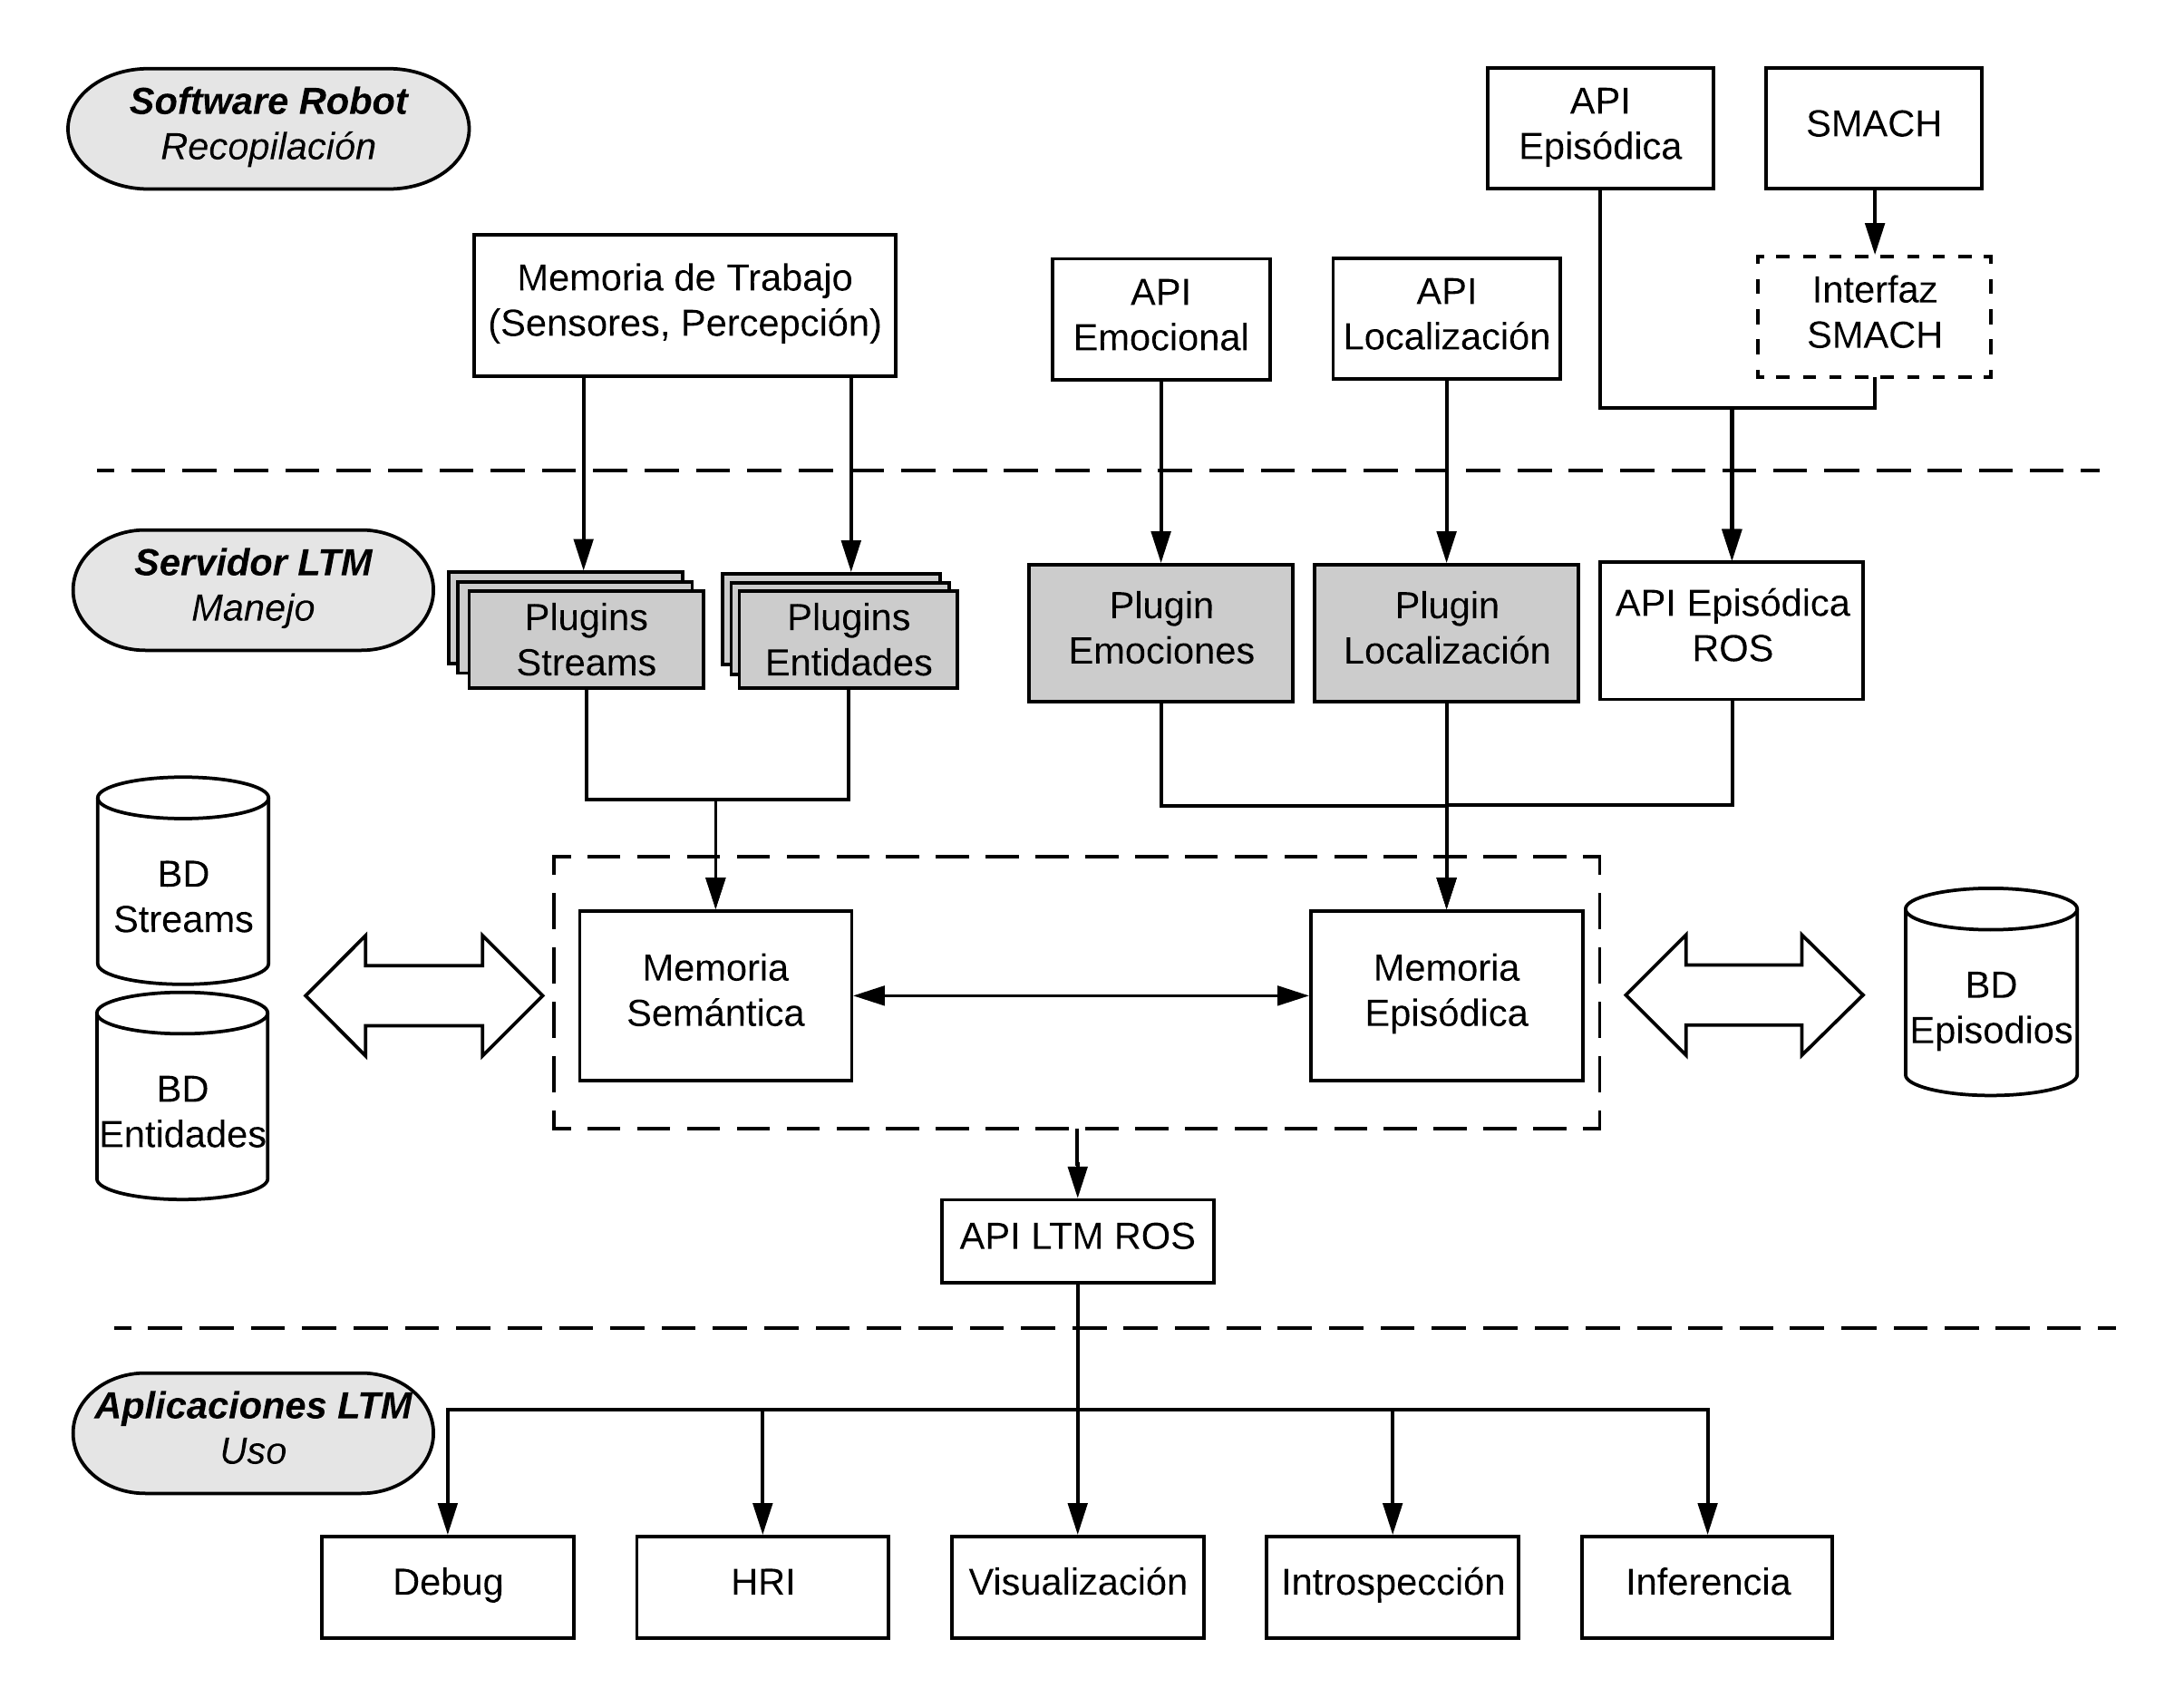
\includegraphics[width=\textwidth]{diagrama-software.png}
	\caption[Diseño del sistema LTM y módulos de software involucrados.]
	{\small Diagrama con el diseño del sistema LTM y los módulos de software involucrados. La zona superior indica todos los módulos de software del robot necesarios para proveer información al sistema LTM. En plomo se presentan los componentes que debe implementar el usuario, que sirven como interfaz entre el robot y el servidor, para la recopilación de información. En la zona central se realiza el manejo y almacenamiento de la información episódica. En la zona inferior, el servidor se comunica mediante una API ROS con las aplicaciones LTM implementadas por el usuario.}
	\label{img:diagrama-software}
\end{figure}


%% =============================================================================
%% =============================================================================
%% =============================================================================
\subsection{Memoria episódica}
%% =============================================================================
%% =============================================================================
%% =============================================================================

En esta sección se describe el diseño del mecanismo para la recolección de episodios, sus datos a partir de plugins y la actualización de relevancias episódicas.

\subsubsection{Recopilación de episodios}

Como se muestra en la Figura~\ref{img:diagrama-software}, el servidor depende de una API episódica para la adquisición de episodios. El diseño propuesto almacena episodios en dos etapas: registro y término, mediante una API ROS basada en servicios. Como lo indica el diagrama, el servidor se comunica con cada plugin para recopilar la información episódica y semántica necesaria.

\ltmconcept{Registro}
En esta etapa, el usuario debe indicar el inicio de un nuevo episodio. Luego, el servidor se encarga de registrar el episodio, generando un identificador único, el que es retornado al usuario. Ya que el sistema debe soportar anidamiento y transposición, pueden haber muchos episodios registrados simultáneamente. 

Durante el registro se debe indicar el tipo de episodio a introducir (hoja o nodo). Si el episodio es de tipo hoja, se notifica a todos los plugins, para que consideren el nuevo episodio como activo e inicien las tareas de recopilación de información. De acuerdo al diseño episódico, no se debe recopilar información para episodios nodo.

\ltmconcept{Término}
Una vez que el episodio ha concluido, el usuario debe notificar al servidor sobre ésto, indicando el identificador del padre, los \textit{tags} asociados y los metadatos episódicos que desee almacenar.

Tras recibir la notificación, el servidor recolecta información episódica desde cada plugin, almacena el episodio en la base de datos y lo marca como inactivo. En caso de ya no haber episodios activos, cada plugin es notificado para dejar de recopilar información.


\subsubsection{Plugin: \textit{Where}}
%% =============================================================================

En cuanto a la recopilación de la ubicación del robot, dato episódico \textit{Where}, el cómo se obtiene la información depende totalmente del usuario y la API de localización utilizada en el robot objetivo (ver diseño episódico en la Sección~\ref{sec:design_ep_where}). Sin embargo, de acuerdo a la sección anterior, el plugin debe proveer las funcionalidades de registro y adquisición de información.

Se propone la siguiente estrategia para la implementación del plugin: recopilar periódicamente el posicionamiento del robot, mientras hayan episodios activos; cuando el servidor necesite la información, se debe proveer un listado con cada ubicación y su instante de tiempo, según el formato estudiado en el diseño episódico del campo \textit{Where}; la lista debe estar restringida a los tiempos de inicio y fin del episodio en consideración.


\subsubsection{Plugin: Emociones}
%% =============================================================================

Los requerimientos y estrategia de funcionamiento propuesta para éste plugin son los mismos que para el plugin \textit{Where}. La información recolectada debe cumplir con el formato propuesto durante el diseño episódico de la Sección~\ref{sec:design_ep_rel_emo}.


\subsubsection{Relevancia histórica y generalizada}
%% =============================================================================

La implementación del servidor debe contar con un proceso automático de actualización de relevancias episódicas, particularmente relevancia histórica y generalizada, según la estrategia descrita en la Sección~\ref{sec:design_ep_rel_hist}. Ya que la cantidad de episodios a actualizar puede ser alta, se debe ejecutar el proceso de actualización cuando el robot no esté en funcionamiento, lo que se traduce en un umbral sobre el porcentaje de recursos disponibles en el sistema. El umbral puede ser escogido por el usuario.


%% =============================================================================
%% =============================================================================
%% =============================================================================
\subsection{Memoria semántica}\label{sec:design_server_semantic_plugins}
%% =============================================================================
%% =============================================================================
%% =============================================================================

En esta sección se describe el diseño de los mecanismos para la recolección de información sobre entidades y \textit{streams}, a través de los plugins respectivos. Se revisan los requerimientos de cada plugin, las estrategias de implementación, el manejo de las colecciones de mensajes y la API ROS que provee el servidor.


\subsubsection{Plugins: \textit{Streams}}
%% =============================================================================

\ltmconcept{Requerimientos}
De acuerdo al diseño para el campo \textit{What}, revisado en la Sección~\ref{sec:design_ep_what}, el primer requisito para la definición de un \textit{stream} es la asignación de un mensaje ROS que lo represente. El mensaje además debe incluir un campo para almacenar metadatos episódicos utilizados por el servidor (id del mensaje, id del episodio y lapso de tiempo). Luego, cada plugin debe indicar el mensaje ROS sobre el que operará.

Este tipo de plugins debe implementar 4 funcionalidades. Proveer un método para el registro de un nuevo episodio y uno para la recolección de la información por el servidor. Además, debe indicar cuales de los campos del mensaje deben ser considerados para ser indexados por la base de datos, pues el resto del mensaje se almacena como objeto binario. Finalmente, debe proveer un método para la degradación del mensaje, por motivos de olvido o escasez de recursos.

\ltmconcept{Estrategia}
El servidor notificará a los plugins por cada nuevo episodio. La estrategia propuesta es mantener un \textit{buffer} circular con información reciente, indexada por su instante de tiempo. Cuando el servidor solicite los datos de un episodio, el plugin genera un \textit{stream} que contiene un listado con mensajes que sucedieron en el periodo del episodio. En el caso de no haber episodios activos, el plugin se debe cerrar sus conexiones ROS, para restringir el uso de recursos.

\ltmconcept{Base de datos}
La implementación del sistema LTM debe manejar automáticamente la colección de mensajes de cada \textit{stream}, por lo que el usuario no debe tener acceso a la base de datos desde el plugin. Así, el servidor se encarga de mantener la consistencia de la información de forma centralizada, evitando delegar ese trabajo a cada usuario y limitando los posibles errores.

\ltmconcept{API ROS}
De la misma forma, el servidor debe proveer automáticamente una API ROS para las operaciones CRUD de cada plugin. Así, se asegura la homogeneidad de la API y se evita agregar otra responsabilidad al usuario. 


\subsubsection{Plugins: Entidades}
%% =============================================================================

\ltmconcept{Requerimientos}
De manera similar al caso de los \textit{streams}, el usuario debe definir un mensaje ROS que represente la entidad de interés. El mensaje debe incluir un campo para almacenar metadatos episódicos utilizados por el servidor. Luego, cada plugin debe indicar el mensaje ROS sobre el que operará.

Ya que el registro de entidades es manejado de manera desacoplada respecto a los episodios (ver Figura~\ref{img:episodes-and-semantic-data}), los métodos que debe proveer el usuario difieren de los utilizados para \textit{streams}. Se deben implementar 4 funcionalidades:
\begin{itemize}
\item Se debe indicar cuales son los campos de interés a ser considerados para ser indexados por la base de datos, pues el resto es almacenado como un objeto binario.
\item Debe proveer un método que permita identificar los campos que han sido modificados entre 2 entidades. El servidor lo utilizará para generar un registro de cambios y mantener el historial.
\item Debe notificar al servidor por cada nuevo registro de una entidad. El servidor verificará los cambios y actualizará el registro de ser necesario.
\item Debe proveer un método para actualizar una entidad, con los campos de otra más actual. El servidor utilizará esta funcionalidad para reconstruir entidades a partir del registro histórico.
\end{itemize}
Cada una de las funcionalidades requeridas es simple de implementar y mantener, las que se reducen a la asignación y comparación de los campos de la entidad definida por el usuario.

\ltmconcept{Estrategia}
El plugin debe estar siempre en funcionamiento, recopilando información a partir de la STM del robot, a pesar de que no existan episodios activos. Cada nueva entidad, o cambio en una ya existente debe ser notificada al servidor, para actualizar los registros de la base de datos. 

En este caso, el registro de nuevos episodios y la recolección de cambios del historial es manejada automáticamente por el servidor, sin requerir intervención del usuario. La estrategia a utilizar es la siguiente. En caso de haber episodios activos, el servidor crea un listado con los identificadores de las entidades modificadas y los registros correspondientes del historial. Cuando el servidor solicita la recolección, se entregan todos los cambios ocurridos en el rango temporal del episodio.

\ltmconcept{Base de datos}
Análogamente al caso de los \textit{streams}, el servidor debe manejar automáticamente la colección de mensajes de cada entidad, por lo que el usuario no debe tener acceso a la base de datos desde el plugin. De esta forma, el servidor se encarga de mantener la consistencia de los registros y el historial de entidades.

\ltmconcept{API ROS}
Asimismo, el servidor debe proveer automáticamente una API ROS para las operaciones CRUD de cada plugin, asegurando la homogeneidad de la API y evitando agregar otra responsabilidad al usuario. 



%% =============================================================================
%% =============================================================================

%% =============================================================================
%% =============================================================================

%% =============================================================================
%% =============================================================================

%% =============================================================================
%% =============================================================================
%% =============================================================================
\section{Diseño de Módulos Específicos para Bender}\label{sec:design_bender}
%% =============================================================================
%% =============================================================================
%% =============================================================================

Según especifican los requisitos \RSlabel{25} y \RSlabel{26}, el proyecto debe ser integrado al robot Bender. Para esto, se debe implementar un módulo que permita recolectar episodios desde SMACH, e implementaciones de cada plugin requerido por el servidor. A continuación se describe el diseño de los componentes a implementar: la interfaz para recolectar episodios, la posición del robot y sus emociones, junto a los plugins para la recolección de \textit{streams} y entidades a partir de la memoria de trabajo de Bender. 

Cada uno de los módulos presentados a continuación cumple una doble funcionalidad. En primer lugar, cumplen con el requisito del diseño de componentes orientados a robots de servicio doméstico, enfocados en el robot Bender. Además, sirven como ejemplo para el diseño e implementación de nuevas funcionalidades requeridas a futuro para otras plataformas.

%% =============================================================================
%% =============================================================================
%% =============================================================================
\subsection{Recolección de episodios: SMACH}
%% =============================================================================
%% =============================================================================
%% =============================================================================

\ltmconcept{SMACH}
El módulo específico más importante a implementar corresponde al encargado de generar episodios a partir del funcionamiento del robot, para luego entregarlos al servidor LTM. Como se explica en la Sección~\ref{sec:URF}, en Bender se utiliza la librería SMACH para la definición y ejecución de las máquinas de estado encargadas de encadenar rutinas simples, para generar comportamientos complejos.

\ltmconcept{Información episódica}
A partir de SMACH se puede obtener parte del conocimiento episódico requerido para la definición de un episodio. Desde el punto de vista de sus transiciones, las máquinas de estado están estructuradas en forma de grafo, estableciendo un inicio y fin temporal para cada estado. Conceptualmente, las máquinas se estructuran en forma de árboles, donde cada maquina de estado puede ser contenida por otra, lo que representa el anidamiento episódico. Luego, SMACH provee una forma de conocimiento episódico, capaz de representar información temporal (\textit{When}) y las relaciones de anidamiento episódico (referencias padre-hijo). Finalmente, ya que cada máquina de estado está asociada a una capacidad o contexto, se puede utilizar esa información para obtener los \textit{tags} requeridos para marcar cada episodio.

\ltmconcept{Funcionamiento}
La interfaz episódica diseñada tiene 2 etapas importantes. En primer lugar, el durante la programación de la máquina, el desarrollador debe indicar que estados considera almacenar como episodio, en caso que sean ejecutados. Además, para cada estado marcado se debe indicar una lista de \textit{tags} que describan brevemente el estado. La segunda etapa ocurre durante el funcionamiento de la máquina de estado, y realiza las tareas de registrar e insertar el episodio en el servidor.

\ltmconcept{Estabilidad de la implementación}
La ejecución ininterrumpida de SMACH durante una rutina es crucial para el desempeño del robot. Si la librería deja de funcionar repentinamente o se detiene continuamente, el robot se detendrá o tomará mucho tiempo en realizar sus tareas, lo que durante una competencia puede tener pésimas consecuencias para el equipo. Es por esto, que la implementación de la interfaz entre el servidor LTM y SMACH debe ser estable. Particularmente, es de vital importancia que el funcionamiento de SMACH no se vea afectado por la implementación, independientemente de si ésta tiene problemas en su ejecución. 

\ltmconcept{Intrusividad}
Por otro lado, la implementación debe minimizar las modificaciones a la librería SMACH y a las máquinas de estado ya implementadas. En primer lugar, si se modifica la librería SMACH, el equipo tendrá que agregar una copia de ésta y mantenerla a futuro, para lo que no hay personal ni tiempo suficiente. Segundo, el robot dispone de muchas máquinas de estado, las que deberán ser actualizadas para agregar la funcionalidad de la interfaz episódica. Por lo tanto, se toman las siguientes decisiones:
\begin{itemize}
\item La librería SMACH no puede ser modificada para la implementación de la interfaz.
\item Las modificaciones a las máquinas de estado deben ser mínimas y opcionales. Esto permitirá ir agregando soporte LTM de manera gradual al robot.
\end{itemize}


%% =============================================================================
%% =============================================================================
%% =============================================================================
\subsection{Recolección de dato episódico: \textit{Where}}
%% =============================================================================
%% =============================================================================
%% =============================================================================

\ltmconcept{Propuesta}
Se debe implementar un plugin para Bender capaz de proveer la posición del robot durante cada episodio, según los requerimientos especificados en la Sección~\ref{sec:design-server}. Por motivos prácticos, se consideran dos versiones a implementar, una con información falsa, y otra capaz de obtener datos reales desde el robot.

\ltmconcept{Versión de prueba} 
Debe proveer datos generados aleatoriamente para cada uno de los campos del mensaje \textit{Where}. La motivación para esto, es poder realizar pruebas durante la implementación del sistema y poder ejecutar validaciones que no precisen de la ubicación real del robot. Además, el plugin permite minimizar el uso del robot real para la implementación y validación del proyecto, pues el robot es un recurso compartido en el equipo de trabajo y su uso implica costos altos en términos de tiempo.

\ltmconcept{Versión en Bender}
Debe ser integrada en el software del robot, a través de la API para la obtención de su ubicación. Se utilizará la estrategia de funcionamiento recomendada en la Sección~\ref{sec:design_ep_where}. El plugin deberá recopilar información periódicamente para cada uno de los campos del mensaje \textit{Where}. Se deberá proveer un listado temporalmente ordenado de las ubicaciones recopiladas. Para disminuir el uso de recursos, solamente se deben recopilar posiciones cuando hayan episodios registrados como activos en el servidor.


%% =============================================================================
%% =============================================================================
%% =============================================================================
\subsection{Recolección de dato episódico: Emociones}
%% =============================================================================
%% =============================================================================
%% =============================================================================

\ltmconcept{Propuesta}
Este plugin está encargado de proveer las emociones registradas por el robot durante cada episodio, según los requerimientos especificados en la Sección~\ref{sec:design-server}. En este caso, también se consideran dos versiones a implementar, una que provee datos falsos, y otra capaz de obtener datos reales desde el robot. Ambas versiones deben recopilar datos para cada uno de los campos del mensaje emocional.

\ltmconcept{Versión de prueba}
Debe proveer datos generados aleatoriamente para cada uno de los campos emocionales. Similarmente al plugin para \textit{Where}, éste permite realizar pruebas durante la implementación del sistema y ejecutar validaciones que no precisen de la emoción real del robot, mientras se minimiza el uso del robot. Sin embargo, la razón principal para su implementación es que actualmente el robot no cuenta con un sistema de emociones.

\ltmconcept{Versión en Bender}
Esta versión debe ser integrada con el software del robot, una vez que se haya implementado el sistema emocional. Para ésto, se utilizará la estrategia de funcionamiento recomendada en la Sección~\ref{sec:design_ep_rel_emo}. El plugin deberá recopilar información periódicamente sobre las emociones del robot. Una vez que el servidor notifique la finalización del episodio, el plugin debe proveer un mensaje emocional con los valores máximos percibidos para cada entidad. Además, para disminuir el uso de recursos, solamente se debe recopilar información cuando hayan episodios registrados como activos en el servidor.

\todofinal{Sobre módulos emocionales en bender.}
%\subsubsection{Modulo emocional: A}
%%% =============================================================================
%
%\subsubsection{Modulo emocional: B}
%%% =============================================================================
%
%\subsubsection{Modulo emocional: C}
%%% =============================================================================
%
%\subsubsection{Modulo emocional: servidor de emociones}
%%% =============================================================================


%% =============================================================================
%% =============================================================================
%% =============================================================================
\subsection{Plugin para streams: Imágenes}
%% =============================================================================
%% =============================================================================
%% =============================================================================

\ltmconcept{Propuesta}
Para los plugins encargados de proveer \textit{streams} de datos se escogió solamente la recopilación de imágenes. Bender dispone de variados datos en su memoria de trabajo que son candidatos para ser almacenados en la memoria semántica, como por ejemplo: el sonido percibido en su micrófono, las nubes de puntos 3D percibidas por su sensor de profundidad, o los posiciones de sus efectores. Sin embargo, el almacenamiento de imágenes es muy útil, pues sirve para la demostración final, permite visualizar lo sucedido en el episodio, y la implementación puede servir para otras plataformas, pues las cámaras de video son un sensor muy común en las plataformas robóticas domésticas. Por motivos prácticos, se consideran dos versiones a implementar, una con información ficticia y otra que recopila datos desde el robot real.

\ltmconcept{Estrategia}
Se utilizará la estrategia de funcionamiento propuesta en la Sección~\ref{sec:design_ep_what}, mediante el uso de un \textit{buffer} para almacenar las últimas imágenes percibidas. Luego, el plugin deberá entregar un vector con las imágenes asociadas al lapso episódico requerido.

\ltmconcept{Versión de prueba}
Debe proveer imágenes obtenidas a partir de un archivo de video. Análogamente a los plugins anteriores, la motivación para esto, es poder acelerar la implementación del proyecto y poder ejecutar validaciones sin requerir el robot real.

\ltmconcept{Versión en Bender}
La segunda versión debe ser integrada en el software robot, utilizando su API ROS para leer imágenes desde sus cámaras de video.

%% =============================================================================
%% =============================================================================
%% =============================================================================
\subsection{Plugins para entidades}
%% =============================================================================
%% =============================================================================
%% =============================================================================
%% =====================================================================================

\ltmconcept{Propuesta}
Se decidió implementar entidades de ``Persona'' y ``Objeto'', pues son las entidades más utilizadas por el robot Bender, y probablemente las más significativas para todo robot de servicio doméstico. Otras entidades de alta relevancia que pueden ser consideradas como trabajo futuro, son las de ``Lugar'' y ``Robot''. De manera similar al caso de los \textit{streams}, se consideran dos versiones a implementar, una capaz de proveer información ficticia sobre cada entidad, y otra encargada de proveer información real recopilada por el robot.

\ltmconcept{Estrategia}
Se utilizará la estrategia de funcionamiento propuesta en la Sección~\ref{sec:design_ep_what}. Para ello, el plugin se debe subscribir a notificaciones sobre cambios en las entidades conocidas. Luego, se deben registrar los cambios percibidos en el historial de la colección, a pesar de que no hayan episodios activos.

\ltmconcept{Versión de prueba}
Se debe implementar un nodo que publique mensajes aleatorios sobre las entidades definidas. El plugin debe subscribirse al tópico asociado, para almacenar registros de las entidades.

\ltmconcept{Versión en Bender}
Se debe implementar un módulo capaz de notificar cambios en las entidades conocidas por el robot, a partir de sus módulos de percepción disponibles. El plugin se debe suscribir al tópico asociado.


